\section{Ablation and Pareto Analysis}
\label{sec:ablation}

\subsection{The Role of Rank-Percentile $B'$}

Without rank-percentile transform (using raw $B$ directly), the unpopularity bonus $1 - B$ becomes saturated near 1 for the long-tail-heavy LFM-1K. This degenerates the reranker to a near-identity transform: low APLT lift, low Gini reduction.

\begin{table}[h]
\caption{Ablation on $B$-transform (LFM-1K, gender, $n=600$).}
\label{tab:ablation-b}
\begin{tabular}{lrrrr}
\toprule
Variant & APLT lift & Gini $\Delta$ & $\Delta$NDCG & $\Delta$MRR \\
\midrule
raw $B$, $\alpha=0.7$ & $+0.005$ & $-0.011$ & $-0.052$ & $-0.069$ \\
raw $B$, $\alpha=0.5$ & $+0.012$ & $-0.024$ & $-0.124$ & $-0.195$ \\
\textbf{rank-$B'$, $\alpha=0.7$, $K'=5$ (v2)} & \textbf{+0.215} & \textbf{$-0.041$} & $-0.076$ & \textbf{$-0.011$} \\
\bottomrule
\end{tabular}
\end{table}

The rank-percentile transform is necessary; raw $B$ produces no meaningful lift even at aggressive $\alpha=0.5$.

\subsection{The Role of Head Protection ($K'$)}

\begin{table}[h]
\caption{Ablation on \texttt{protect\_top} (LFM-1K, gender, rank-$B'$, $\alpha=0.7$).}
\label{tab:ablation-k}
\begin{tabular}{rrrr}
\toprule
$K'$ & $\Delta$MRR & $\Delta$NDCG & $\Delta$APLT \\
\midrule
0 (no protection) & $-0.069$ & $-0.085$ & $+0.225$ \\
3 & $-0.024$ & $-0.080$ & $+0.221$ \\
\textbf{5 (v2 default)} & \textbf{$-0.011$} & $-0.076$ & $+0.215$ \\
10 & $-0.005$ & $-0.071$ & $+0.198$ \\
\bottomrule
\end{tabular}
\end{table}

A modest protection of $K'=5$ recovers ${\sim}\,6$\,pp of MRR loss while sacrificing only $1$\,pp of APLT lift, a clear Pareto-improving operating point.

\subsection{Per-User $\alpha$ Adaptive vs Fixed}

% PLACEHOLDER
[\textbf{Placeholder}: comparison of dynamic $\alpha$ vs fixed $\alpha$ to demonstrate value of user-mainstream-ness adaptation.]

\subsection{Pareto Frontier Scatter}

\begin{figure}[t]
\centering
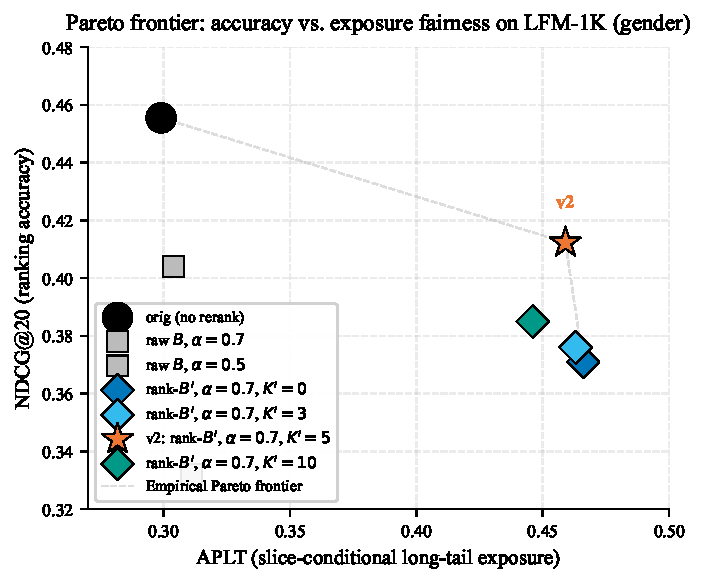
\includegraphics[width=0.95\columnwidth]{figures/fig1_pareto.pdf}
\caption{Pareto frontier on LFM-1K (gender scenario, $n=600$). Each point is a (rerank algorithm, $\alpha$, $K'$) configuration. The original LLM output and v2 (rank-$B'$ + protect\_top=5) jointly define the empirical Pareto frontier; raw-$B$ baselines are dominated.}
\label{fig:pareto}
\end{figure}

Figure~\ref{fig:pareto} situates v2 on the empirical Pareto frontier between accuracy and exposure-fairness. Raw-$B$ baselines fall below the frontier (dominated): rank-$B'$ with $K'=5$ recovers ${\approx}\,90\%$ of the original NDCG while delivering $1.5{\times}$ the APLT.
